% !TEX root = ../5.DOUBLE-PIPE.tex
\section{RESULTS}\label{results-1}

\subsection{Raw Experimental Data}\label{raw-data}

\begin{table}[H]
    \centering
    \caption{Tube B Experimental Data (Flow rates in L/min, Temperatures in $^\circ$C)}
    \label{tab:raw-data-tube-b}
    \resizebox{\textwidth}{!}{
        \begin{tabular}{|c|c|c|c|c|c|c|c|c|c|c|c|c|c|c|c|c|c|c|c|c|}
            \hline
            \textbf{Cold Flow} & \multicolumn{4}{c|}{\textbf{Hot: 4}} & \multicolumn{4}{c|}{\textbf{Hot: 6}} & \multicolumn{4}{c|}{\textbf{Hot: 8}} & \multicolumn{4}{c|}{\textbf{Hot: 10}} & \multicolumn{4}{c|}{\textbf{Hot: 12}}                                                                                                                                                                                                            \\
            \hline
            \textbf{(L/min)}   & $T_{1,in}$                           & $T_{1,out}$                          & $T_{2,in}$                           & $T_{2,out}$                           & $T_{1,in}$                            & $T_{1,out}$ & $T_{2,in}$ & $T_{2,out}$ & $T_{1,in}$ & $T_{1,out}$ & $T_{2,in}$ & $T_{2,out}$ & $T_{1,in}$ & $T_{1,out}$ & $T_{2,in}$ & $T_{2,out}$ & $T_{1,in}$ & $T_{1,out}$ & $T_{2,in}$ & $T_{2,out}$ \\
            \hline
            \textbf{4}         & 54                                   & 49                                   & 34                                   & 40                                    & 59                                    & 54          & 36         & 42          & 64         & 58          & 39         & 45          & 69         & 63          & 40         & 47          & 71         & 66          & 41         & 48          \\ \hline
            \textbf{6}         & 56                                   & 49                                   & 35                                   & 40                                    & 60                                    & 54          & 36         & 42          & 65         & 58          & 38         & 44          & 70         & 63          & 40         & 46          & 71         & 66          & 41         & 47          \\ \hline
            \textbf{8}         & 56                                   & 50                                   & 34                                   & 40                                    & 60                                    & 54          & 36         & 42          & 66         & 58          & 37         & 43          & 70         & 63          & 39         & 44          & 71         & 65          & 40         & 46          \\ \hline
            \textbf{10}        & 57                                   & 50                                   & 34                                   & 40                                    & 62                                    & 54          & 36         & 41          & 67         & 58          & 37         & 42          & 70         & 63          & 39         & 44          & 72         & 65          & 40         & 45          \\ \hline
            \textbf{12}        & 58                                   & 51                                   & 34                                   & 40                                    & 63                                    & 55          & 36         & 41          & 68         & 59          & 37         & 42          & 71         & 63          & 39         & 44          & 72         & 66          & 40         & 45          \\ \hline
        \end{tabular}
    }
\end{table}

\begin{table}[H]
    \centering
    \caption{Tube C$_2$ Experimental Data (Flow rates in L/min, Temperatures in $^\circ$C)}
    \label{tab:raw-data-tube-c}
    \resizebox{\textwidth}{!}{
        \begin{tabular}{|c|c|c|c|c|c|c|c|c|c|c|c|c|c|c|c|c|c|c|c|c|}
            \hline
            \textbf{Cold Flow} & \multicolumn{4}{c|}{\textbf{Hot: 4}} & \multicolumn{4}{c|}{\textbf{Hot: 6}} & \multicolumn{4}{c|}{\textbf{Hot: 8}} & \multicolumn{4}{c|}{\textbf{Hot: 10}} & \multicolumn{4}{c|}{\textbf{Hot: 12}}                                                                                                                                                                                                            \\
            \hline
            \textbf{(L/min)}   & $T_{1,in}$                           & $T_{1,out}$                          & $T_{2,in}$                           & $T_{2,out}$                           & $T_{1,in}$                            & $T_{1,out}$ & $T_{2,in}$ & $T_{2,out}$ & $T_{1,in}$ & $T_{1,out}$ & $T_{2,in}$ & $T_{2,out}$ & $T_{1,in}$ & $T_{1,out}$ & $T_{2,in}$ & $T_{2,out}$ & $T_{1,in}$ & $T_{1,out}$ & $T_{2,in}$ & $T_{2,out}$ \\
            \hline
            \textbf{4}         & 61                                   & 50                                   & 32                                   & 36                                    & 67                                    & 56          & 35         & 39          & 69         & 59          & 37         & 41          & 69         & 61          & 39         & 43          & 71         & 63          & 40         & 44          \\ \hline
            \textbf{6}         & 63                                   & 52                                   & 32                                   & 35                                    & 67                                    & 56          & 34         & 38          & 69         & 59          & 36         & 40          & 70         & 61          & 38         & 42          & 71         & 63          & 40         & 43          \\ \hline
            \textbf{8}         & 65                                   & 53                                   & 32                                   & 35                                    & 67                                    & 56          & 34         & 37          & 70         & 59          & 36         & 40          & 71         & 61          & 38         & 41          & 71         & 62          & 39         & 42          \\ \hline
            \textbf{10}        & 66                                   & 53                                   & 32                                   & 35                                    & 68                                    & 56          & 34         & 37          & 69         & 59          & 36         & 39          & 71         & 61          & 38         & 41          & 72         & 62          & 39         & 41          \\ \hline
            \textbf{12}        & 66                                   & 53                                   & 33                                   & 35                                    & 69                                    & 56          & 34         & 37          & 70         & 59          & 36         & 39          & 71         & 61          & 37         & 40          & 72         & 62          & 38         & 41          \\ \hline
        \end{tabular}
    }
\end{table}

\subsection{Calculated Experimental Results}\label{exp-results}

\subsubsection{Fluid Physical Parameters}\label{fluid-params}

The physical properties of water are interpolated based on the average flow temperature $T_{avg} = (T_{in} + T_{out})/2$.

    {\small
        \setlength{\tabcolsep}{3pt}
        \begin{longtable}{|c|c|c|c|c|c|c|c|c|c|c|}
            \caption{Fluid Parameters - Hot stream - Tube B} \label{tab:params-hot-b}                                                                                                                                               \\ \hline
            \textbf{No.} & \boldmath$G_1$ & \boldmath$G_2$ & \boldmath$T_{1,in}$ & \boldmath$T_{1,out}$ & \boldmath$T_{1,avg}$ & \boldmath$\rho_1$ & \boldmath$C_{p,1}$ & \boldmath$\lambda_1$ & \boldmath$\mu_1$ & \boldmath$Pr_1$ \\
                         & (L/min)        & (L/min)        & ($^\circ$C)         & ($^\circ$C)          & ($^\circ$C)          & (kg/m$^3$)        & (J/kg$\cdot$K)     & (W/m$\cdot$K)        & (Pa$\cdot$s)     &                 \\ \hline
            \endfirsthead
            \multicolumn{11}{c}{{\bfseries \tablename\ \thetable\ -- continued from previous page}}                                                                                                                                 \\ \hline
            \textbf{No.} & \boldmath$G_1$ & \boldmath$G_2$ & \boldmath$T_{1,in}$ & \boldmath$T_{1,out}$ & \boldmath$T_{1,avg}$ & \boldmath$\rho_1$ & \boldmath$C_{p,1}$ & \boldmath$\lambda_1$ & \boldmath$\mu_1$ & \boldmath$Pr_1$ \\
                         & (L/min)        & (L/min)        & ($^\circ$C)         & ($^\circ$C)          & ($^\circ$C)          & (kg/m$^3$)        & (J/kg$\cdot$K)     & (W/m$\cdot$K)        & (Pa$\cdot$s)     &                 \\ \hline
            \endhead
            1            & 4              & 4              & 54                  & 49                   & 51.50                & 987.37            & 4182               & 0.6455               & 5.35e-04         & 3.46            \\
            2            & 4              & 6              & 56                  & 49                   & 52.50                & 986.88            & 4182               & 0.6465               & 5.27e-04         & 3.41            \\
            3            & 4              & 8              & 56                  & 50                   & 53.00                & 986.63            & 4182               & 0.6470               & 5.23e-04         & 3.38            \\
            4            & 4              & 10             & 57                  & 50                   & 53.50                & 986.38            & 4182               & 0.6475               & 5.19e-04         & 3.35            \\
            5            & 4              & 12             & 58                  & 51                   & 54.50                & 985.89            & 4183               & 0.6485               & 5.11e-04         & 3.29            \\ \hline
            6            & 6              & 4              & 59                  & 54                   & 56.50                & 984.92            & 4184               & 0.6505               & 4.95e-04         & 3.18            \\
            7            & 6              & 6              & 60                  & 54                   & 57.00                & 984.67            & 4184               & 0.6510               & 4.91e-04         & 3.15            \\
            8            & 6              & 8              & 60                  & 54                   & 57.00                & 984.67            & 4184               & 0.6510               & 4.91e-04         & 3.15            \\
            9            & 6              & 10             & 62                  & 54                   & 58.00                & 984.18            & 4184               & 0.6520               & 4.83e-04         & 3.09            \\
            10           & 6              & 12             & 63                  & 55                   & 59.00                & 983.69            & 4185               & 0.6530               & 4.75e-04         & 3.04            \\ \hline
            11           & 8              & 4              & 64                  & 58                   & 61.00                & 982.66            & 4186               & 0.6549               & 4.61e-04         & 2.94            \\
            12           & 8              & 6              & 65                  & 58                   & 61.50                & 982.39            & 4186               & 0.6553               & 4.58e-04         & 2.92            \\
            13           & 8              & 8              & 66                  & 58                   & 62.00                & 982.12            & 4186               & 0.6558               & 4.54e-04         & 2.89            \\
            14           & 8              & 10             & 67                  & 58                   & 62.50                & 981.85            & 4186               & 0.6562               & 4.51e-04         & 2.87            \\
            15           & 8              & 12             & 68                  & 59                   & 63.50                & 981.31            & 4187               & 0.6572               & 4.45e-04         & 2.83            \\ \hline
            16           & 10             & 4              & 69                  & 63                   & 66.00                & 979.96            & 4188               & 0.6594               & 4.29e-04         & 2.72            \\
            17           & 10             & 6              & 70                  & 63                   & 66.50                & 979.69            & 4188               & 0.6599               & 4.26e-04         & 2.70            \\
            18           & 10             & 8              & 70                  & 63                   & 66.50                & 979.69            & 4188               & 0.6599               & 4.26e-04         & 2.70            \\
            19           & 10             & 10             & 70                  & 63                   & 66.50                & 979.69            & 4188               & 0.6599               & 4.26e-04         & 2.70            \\
            20           & 10             & 12             & 71                  & 63                   & 67.00                & 979.42            & 4188               & 0.6603               & 4.23e-04         & 2.68            \\ \hline
            21           & 12             & 4              & 71                  & 66                   & 68.50                & 978.61            & 4189               & 0.6617               & 4.13e-04         & 2.61            \\
            22           & 12             & 6              & 71                  & 66                   & 68.50                & 978.61            & 4189               & 0.6617               & 4.13e-04         & 2.61            \\
            23           & 12             & 8              & 71                  & 65                   & 68.00                & 978.88            & 4189               & 0.6612               & 4.17e-04         & 2.64            \\
            24           & 12             & 10             & 72                  & 65                   & 68.50                & 978.61            & 4189               & 0.6617               & 4.13e-04         & 2.61            \\
            25           & 12             & 12             & 72                  & 66                   & 69.00                & 978.34            & 4190               & 0.6621               & 4.10e-04         & 2.59            \\ \hline
        \end{longtable}
    }

    {\small
        \setlength{\tabcolsep}{3pt}
        \begin{longtable}{|c|c|c|c|c|c|c|c|c|c|c|}
            \caption{Fluid Parameters - Cold stream - Tube B} \label{tab:params-cold-b}                                                                                                                                             \\ \hline
            \textbf{No.} & \boldmath$G_1$ & \boldmath$G_2$ & \boldmath$T_{2,in}$ & \boldmath$T_{2,out}$ & \boldmath$T_{2,avg}$ & \boldmath$\rho_2$ & \boldmath$C_{p,2}$ & \boldmath$\lambda_2$ & \boldmath$\mu_2$ & \boldmath$Pr_2$ \\
                         & (L/min)        & (L/min)        & ($^\circ$C)         & ($^\circ$C)          & ($^\circ$C)          & (kg/m$^3$)        & (J/kg$\cdot$K)     & (W/m$\cdot$K)        & (Pa$\cdot$s)     &                 \\ \hline
            \endfirsthead
            \multicolumn{11}{c}{{\bfseries \tablename\ \thetable\ -- continued from previous page}}                                                                                                                                 \\ \hline
            \textbf{No.} & \boldmath$G_1$ & \boldmath$G_2$ & \boldmath$T_{2,in}$ & \boldmath$T_{2,out}$ & \boldmath$T_{2,avg}$ & \boldmath$\rho_2$ & \boldmath$C_{p,2}$ & \boldmath$\lambda_2$ & \boldmath$\mu_2$ & \boldmath$Pr_2$ \\
                         & (L/min)        & (L/min)        & ($^\circ$C)         & ($^\circ$C)          & ($^\circ$C)          & (kg/m$^3$)        & (J/kg$\cdot$K)     & (W/m$\cdot$K)        & (Pa$\cdot$s)     &                 \\ \hline
            \endhead
            1            & 4              & 4              & 34                  & 40                   & 37.00                & 993.25            & 4179               & 0.6262               & 6.97e-04         & 4.65            \\
            2            & 4              & 6              & 35                  & 40                   & 37.50                & 993.08            & 4179               & 0.6270               & 6.89e-04         & 4.60            \\
            3            & 4              & 8              & 34                  & 40                   & 37.00                & 993.25            & 4179               & 0.6262               & 6.97e-04         & 4.65            \\
            4            & 4              & 10             & 34                  & 40                   & 37.00                & 993.25            & 4179               & 0.6262               & 6.97e-04         & 4.65            \\
            5            & 4              & 12             & 34                  & 40                   & 37.00                & 993.25            & 4179               & 0.6262               & 6.97e-04         & 4.65            \\ \hline
            6            & 6              & 4              & 36                  & 42                   & 39.00                & 992.55            & 4179               & 0.6294               & 6.68e-04         & 4.43            \\
            7            & 6              & 6              & 36                  & 42                   & 39.00                & 992.55            & 4179               & 0.6294               & 6.68e-04         & 4.43            \\
            8            & 6              & 8              & 36                  & 42                   & 39.00                & 992.55            & 4179               & 0.6294               & 6.68e-04         & 4.43            \\
            9            & 6              & 10             & 36                  & 41                   & 38.50                & 992.73            & 4179               & 0.6286               & 6.75e-04         & 4.49            \\
            10           & 6              & 12             & 36                  & 41                   & 38.50                & 992.73            & 4179               & 0.6286               & 6.75e-04         & 4.49            \\ \hline
            11           & 8              & 4              & 39                  & 45                   & 42.00                & 991.38            & 4179               & 0.6336               & 6.32e-04         & 4.17            \\
            12           & 8              & 6              & 38                  & 44                   & 41.00                & 991.79            & 4179               & 0.6323               & 6.42e-04         & 4.24            \\
            13           & 8              & 8              & 37                  & 43                   & 40.00                & 992.20            & 4179               & 0.6310               & 6.53e-04         & 4.32            \\
            14           & 8              & 10             & 37                  & 42                   & 39.50                & 992.38            & 4179               & 0.6302               & 6.60e-04         & 4.38            \\
            15           & 8              & 12             & 37                  & 42                   & 39.50                & 992.38            & 4179               & 0.6302               & 6.60e-04         & 4.38            \\ \hline
            16           & 10             & 4              & 40                  & 47                   & 43.50                & 990.76            & 4180               & 0.6356               & 6.16e-04         & 4.05            \\
            17           & 10             & 6              & 40                  & 46                   & 43.00                & 990.97            & 4180               & 0.6349               & 6.21e-04         & 4.09            \\
            18           & 10             & 8              & 39                  & 44                   & 41.50                & 991.59            & 4179               & 0.6330               & 6.37e-04         & 4.20            \\
            19           & 10             & 10             & 39                  & 44                   & 41.50                & 991.59            & 4179               & 0.6330               & 6.37e-04         & 4.20            \\
            20           & 10             & 12             & 39                  & 44                   & 41.50                & 991.59            & 4179               & 0.6330               & 6.37e-04         & 4.20            \\ \hline
            21           & 12             & 4              & 41                  & 48                   & 44.50                & 990.36            & 4180               & 0.6369               & 6.05e-04         & 3.97            \\
            22           & 12             & 6              & 41                  & 47                   & 44.00                & 990.56            & 4180               & 0.6362               & 6.11e-04         & 4.01            \\
            23           & 12             & 8              & 40                  & 46                   & 43.00                & 990.97            & 4180               & 0.6349               & 6.21e-04         & 4.09            \\
            24           & 12             & 10             & 40                  & 45                   & 42.50                & 991.18            & 4180               & 0.6342               & 6.26e-04         & 4.13            \\
            25           & 12             & 12             & 40                  & 45                   & 42.50                & 991.18            & 4180               & 0.6342               & 6.26e-04         & 4.13            \\ \hline
        \end{longtable}
    }

    {\small
        \setlength{\tabcolsep}{3pt}
        \begin{longtable}{|c|c|c|c|c|c|c|c|c|c|c|}
            \caption{Fluid Parameters - Hot stream - Tube C} \label{tab:params-hot-c}                                                                                                                                               \\ \hline
            \textbf{No.} & \boldmath$G_1$ & \boldmath$G_2$ & \boldmath$T_{1,in}$ & \boldmath$T_{1,out}$ & \boldmath$T_{1,avg}$ & \boldmath$\rho_1$ & \boldmath$C_{p,1}$ & \boldmath$\lambda_1$ & \boldmath$\mu_1$ & \boldmath$Pr_1$ \\
                         & (L/min)        & (L/min)        & ($^\circ$C)         & ($^\circ$C)          & ($^\circ$C)          & (kg/m$^3$)        & (J/kg$\cdot$K)     & (W/m$\cdot$K)        & (Pa$\cdot$s)     &                 \\ \hline
            \endfirsthead
            \multicolumn{11}{c}{{\bfseries \tablename\ \thetable\ -- continued from previous page}}                                                                                                                                 \\ \hline
            \textbf{No.} & \boldmath$G_1$ & \boldmath$G_2$ & \boldmath$T_{1,in}$ & \boldmath$T_{1,out}$ & \boldmath$T_{1,avg}$ & \boldmath$\rho_1$ & \boldmath$C_{p,1}$ & \boldmath$\lambda_1$ & \boldmath$\mu_1$ & \boldmath$Pr_1$ \\
                         & (L/min)        & (L/min)        & ($^\circ$C)         & ($^\circ$C)          & ($^\circ$C)          & (kg/m$^3$)        & (J/kg$\cdot$K)     & (W/m$\cdot$K)        & (Pa$\cdot$s)     &                 \\ \hline
            \endhead
            1            & 4              & 4              & 61                  & 50                   & 55.50                & 985.41            & 4183               & 0.6495               & 5.03e-04         & 3.24            \\
            2            & 4              & 6              & 63                  & 52                   & 57.50                & 984.43            & 4184               & 0.6515               & 4.87e-04         & 3.12            \\
            3            & 4              & 8              & 65                  & 53                   & 59.00                & 983.69            & 4185               & 0.6530               & 4.75e-04         & 3.04            \\
            4            & 4              & 10             & 66                  & 53                   & 59.50                & 983.45            & 4185               & 0.6535               & 4.71e-04         & 3.01            \\
            5            & 4              & 12             & 66                  & 53                   & 59.50                & 983.45            & 4185               & 0.6535               & 4.71e-04         & 3.01            \\ \hline
            6            & 6              & 4              & 67                  & 56                   & 61.50                & 982.39            & 4186               & 0.6553               & 4.58e-04         & 2.92            \\
            7            & 6              & 6              & 67                  & 56                   & 61.50                & 982.39            & 4186               & 0.6553               & 4.58e-04         & 2.92            \\
            8            & 6              & 8              & 67                  & 56                   & 61.50                & 982.39            & 4186               & 0.6553               & 4.58e-04         & 2.92            \\
            9            & 6              & 10             & 68                  & 56                   & 62.00                & 982.12            & 4186               & 0.6558               & 4.54e-04         & 2.89            \\
            10           & 6              & 12             & 69                  & 56                   & 62.50                & 981.85            & 4186               & 0.6562               & 4.51e-04         & 2.87            \\ \hline
            11           & 8              & 4              & 69                  & 59                   & 64.00                & 981.04            & 4187               & 0.6576               & 4.42e-04         & 2.81            \\
            12           & 8              & 6              & 69                  & 59                   & 64.00                & 981.04            & 4187               & 0.6576               & 4.42e-04         & 2.81            \\
            13           & 8              & 8              & 70                  & 59                   & 64.50                & 980.77            & 4187               & 0.6581               & 4.39e-04         & 2.79            \\
            14           & 8              & 10             & 69                  & 59                   & 64.00                & 981.04            & 4187               & 0.6576               & 4.42e-04         & 2.81            \\
            15           & 8              & 12             & 70                  & 59                   & 64.50                & 980.77            & 4187               & 0.6581               & 4.39e-04         & 2.79            \\ \hline
            16           & 10             & 4              & 69                  & 61                   & 65.00                & 980.50            & 4188               & 0.6585               & 4.36e-04         & 2.76            \\
            17           & 10             & 6              & 70                  & 61                   & 65.50                & 980.23            & 4188               & 0.6590               & 4.32e-04         & 2.74            \\
            18           & 10             & 8              & 71                  & 61                   & 66.00                & 979.96            & 4188               & 0.6594               & 4.29e-04         & 2.72            \\
            19           & 10             & 10             & 71                  & 61                   & 66.00                & 979.96            & 4188               & 0.6594               & 4.29e-04         & 2.72            \\
            20           & 10             & 12             & 71                  & 61                   & 66.00                & 979.96            & 4188               & 0.6594               & 4.29e-04         & 2.72            \\ \hline
            21           & 12             & 4              & 71                  & 63                   & 67.00                & 979.42            & 4188               & 0.6603               & 4.23e-04         & 2.68            \\
            22           & 12             & 6              & 71                  & 63                   & 67.00                & 979.42            & 4188               & 0.6603               & 4.23e-04         & 2.68            \\
            23           & 12             & 8              & 71                  & 62                   & 66.50                & 979.69            & 4188               & 0.6599               & 4.26e-04         & 2.70            \\
            24           & 12             & 10             & 72                  & 62                   & 67.00                & 979.42            & 4188               & 0.6603               & 4.23e-04         & 2.68            \\
            25           & 12             & 12             & 72                  & 62                   & 67.00                & 979.42            & 4188               & 0.6603               & 4.23e-04         & 2.68            \\ \hline
        \end{longtable}
    }

    {\small
        \setlength{\tabcolsep}{3pt}
        \begin{longtable}{|c|c|c|c|c|c|c|c|c|c|c|}
            \caption{Fluid Parameters - Cold stream - Tube C} \label{tab:params-cold-c}                                                                                                                                             \\ \hline
            \textbf{No.} & \boldmath$G_1$ & \boldmath$G_2$ & \boldmath$T_{2,in}$ & \boldmath$T_{2,out}$ & \boldmath$T_{2,avg}$ & \boldmath$\rho_2$ & \boldmath$C_{p,2}$ & \boldmath$\lambda_2$ & \boldmath$\mu_2$ & \boldmath$Pr_2$ \\
                         & (L/min)        & (L/min)        & ($^\circ$C)         & ($^\circ$C)          & ($^\circ$C)          & (kg/m$^3$)        & (J/kg$\cdot$K)     & (W/m$\cdot$K)        & (Pa$\cdot$s)     &                 \\ \hline
            \endfirsthead
            \multicolumn{11}{c}{{\bfseries \tablename\ \thetable\ -- continued from previous page}}                                                                                                                                 \\ \hline
            \textbf{No.} & \boldmath$G_1$ & \boldmath$G_2$ & \boldmath$T_{2,in}$ & \boldmath$T_{2,out}$ & \boldmath$T_{2,avg}$ & \boldmath$\rho_2$ & \boldmath$C_{p,2}$ & \boldmath$\lambda_2$ & \boldmath$\mu_2$ & \boldmath$Pr_2$ \\
                         & (L/min)        & (L/min)        & ($^\circ$C)         & ($^\circ$C)          & ($^\circ$C)          & (kg/m$^3$)        & (J/kg$\cdot$K)     & (W/m$\cdot$K)        & (Pa$\cdot$s)     &                 \\ \hline
            \endhead
            1            & 4              & 4              & 32                  & 36                   & 34.00                & 994.30            & 4178               & 0.6214               & 7.40e-04         & 4.98            \\
            2            & 4              & 6              & 32                  & 35                   & 33.50                & 994.48            & 4178               & 0.6206               & 7.47e-04         & 5.04            \\
            3            & 4              & 8              & 32                  & 35                   & 33.50                & 994.48            & 4178               & 0.6206               & 7.47e-04         & 5.04            \\
            4            & 4              & 10             & 32                  & 35                   & 33.50                & 994.48            & 4178               & 0.6206               & 7.47e-04         & 5.04            \\
            5            & 4              & 12             & 33                  & 35                   & 34.00                & 994.30            & 4178               & 0.6214               & 7.40e-04         & 4.98            \\ \hline
            6            & 6              & 4              & 35                  & 39                   & 37.00                & 993.25            & 4179               & 0.6262               & 6.97e-04         & 4.65            \\
            7            & 6              & 6              & 34                  & 38                   & 36.00                & 993.60            & 4179               & 0.6246               & 7.11e-04         & 4.76            \\
            8            & 6              & 8              & 34                  & 37                   & 35.50                & 993.78            & 4179               & 0.6238               & 7.18e-04         & 4.82            \\
            9            & 6              & 10             & 34                  & 37                   & 35.50                & 993.78            & 4179               & 0.6238               & 7.18e-04         & 4.82            \\
            10           & 6              & 12             & 34                  & 37                   & 35.50                & 993.78            & 4179               & 0.6238               & 7.18e-04         & 4.82            \\ \hline
            11           & 8              & 4              & 37                  & 41                   & 39.00                & 992.55            & 4179               & 0.6294               & 6.68e-04         & 4.43            \\
            12           & 8              & 6              & 36                  & 40                   & 38.00                & 992.90            & 4179               & 0.6278               & 6.82e-04         & 4.54            \\
            13           & 8              & 8              & 36                  & 40                   & 38.00                & 992.90            & 4179               & 0.6278               & 6.82e-04         & 4.54            \\
            14           & 8              & 10             & 36                  & 39                   & 37.50                & 993.08            & 4179               & 0.6270               & 6.89e-04         & 4.60            \\
            15           & 8              & 12             & 36                  & 39                   & 37.50                & 993.08            & 4179               & 0.6270               & 6.89e-04         & 4.60            \\ \hline
            16           & 10             & 4              & 39                  & 43                   & 41.00                & 991.79            & 4179               & 0.6323               & 6.42e-04         & 4.24            \\
            17           & 10             & 6              & 38                  & 42                   & 40.00                & 992.20            & 4179               & 0.6310               & 6.53e-04         & 4.32            \\
            18           & 10             & 8              & 38                  & 41                   & 39.50                & 992.38            & 4179               & 0.6302               & 6.60e-04         & 4.38            \\
            19           & 10             & 10             & 38                  & 41                   & 39.50                & 992.38            & 4179               & 0.6302               & 6.60e-04         & 4.38            \\
            20           & 10             & 12             & 37                  & 40                   & 38.50                & 992.73            & 4179               & 0.6286               & 6.75e-04         & 4.49            \\ \hline
            21           & 12             & 4              & 40                  & 44                   & 42.00                & 991.38            & 4179               & 0.6336               & 6.32e-04         & 4.17            \\
            22           & 12             & 6              & 40                  & 43                   & 41.50                & 991.59            & 4179               & 0.6330               & 6.37e-04         & 4.20            \\
            23           & 12             & 8              & 39                  & 42                   & 40.50                & 992.00            & 4179               & 0.6317               & 6.48e-04         & 4.28            \\
            24           & 12             & 10             & 39                  & 41                   & 40.00                & 992.20            & 4179               & 0.6310               & 6.53e-04         & 4.32            \\
            25           & 12             & 12             & 38                  & 41                   & 39.50                & 992.38            & 4179               & 0.6302               & 6.60e-04         & 4.38            \\ \hline
        \end{longtable}
    }

\subsubsection{Heat Balance and Loss}\label{heat-balance}

The heat transfer rate for the hot stream ($Q_1$) and cold stream ($Q_2$) are calculated as:
\begin{equation}
    Q = \dot{m} C_p (T_{in} - T_{out}) = \rho G_{L/min} \frac{10^{-3}}{60} C_p \Delta T
\end{equation}

\textbf{Sample Calculation (Row 1, Tube B):}
\begin{itemize}
    \item $Q_1 = 987.37 \times 4 \times \frac{10^{-3}}{60} \times 4182 \times (54 - 49) = 1376.26 \, \text{W}$
    \item $Q_2 = 993.25 \times 4 \times \frac{10^{-3}}{60} \times 4179 \times (40 - 34) = 1660.20 \, \text{W}$
    \item $Q_{loss} = Q_1 - Q_2 = 1376.26 - 1660.20 = -283.94 \, \text{W}$
\end{itemize}

{\small
\setlength{\tabcolsep}{3pt}
\begin{longtable}{|c|c|c|c|c|c|}
    \caption{Heat balance - Tube B} \label{tab:q-b}                                        \\ \hline
    \textbf{No.} & \shortstack{\boldmath$\Delta T_1$                                       \\ ($^\circ$C)} & \shortstack{\boldmath$Q_1$ \\ (W)} & \shortstack{\boldmath$\Delta T_2$ \\ ($^\circ$C)} & \shortstack{\boldmath$Q_2$ \\ (W)} & \shortstack{\boldmath$Q_{loss}$ \\ (W)} \\ \hline
    \endfirsthead
    \multicolumn{6}{c}{{\bfseries \tablename\ \thetable\ -- continued from previous page}} \\ \hline
    \textbf{No.} & \shortstack{\boldmath$\Delta T_1$                                       \\ ($^\circ$C)} & \shortstack{\boldmath$Q_1$ \\ (W)} & \shortstack{\boldmath$\Delta T_2$ \\ ($^\circ$C)} & \shortstack{\boldmath$Q_2$ \\ (W)} & \shortstack{\boldmath$Q_{loss}$ \\ (W)} \\ \hline
    \endhead
    1            & 5                                 & 1376.26 & 6 & 1660.20 & -283.94     \\
    2            & 7                                 & 1925.99 & 5 & 2074.91 & -148.92     \\
    3            & 6                                 & 1650.51 & 6 & 3320.40 & -1669.88    \\
    4            & 7                                 & 1925.21 & 6 & 4150.49 & -2225.28    \\
    5            & 7                                 & 1924.44 & 6 & 4980.59 & -3056.15    \\ \hline
    6            & 5                                 & 2060.25 & 6 & 1659.11 & 401.14      \\
    7            & 6                                 & 2471.80 & 6 & 2488.66 & -16.86      \\
    8            & 6                                 & 2471.80 & 6 & 3318.21 & -846.42     \\
    9            & 8                                 & 3294.40 & 5 & 3457.04 & -162.64     \\
    10           & 8                                 & 3293.08 & 5 & 4148.45 & -855.37     \\ \hline
    11           & 6                                 & 3290.34 & 6 & 1657.35 & 1632.99     \\
    12           & 7                                 & 3837.90 & 6 & 2486.93 & 1350.97     \\
    13           & 8                                 & 4385.23 & 6 & 3317.12 & 1068.11     \\
    14           & 9                                 & 4932.32 & 5 & 3455.90 & 1476.42     \\
    15           & 9                                 & 4930.20 & 5 & 4147.09 & 783.11      \\ \hline
    16           & 6                                 & 4104.07 & 7 & 1932.51 & 2171.56     \\
    17           & 7                                 & 4787.05 & 6 & 2485.11 & 2301.94     \\
    18           & 7                                 & 4787.05 & 5 & 2762.75 & 2024.30     \\
    19           & 7                                 & 4787.05 & 5 & 3453.44 & 1333.61     \\
    20           & 8                                 & 5469.73 & 5 & 4144.13 & 1325.60     \\ \hline
    21           & 5                                 & 4099.64 & 7 & 1931.81 & 2167.84     \\
    22           & 5                                 & 4099.64 & 6 & 2484.21 & 1615.44     \\
    23           & 6                                 & 4920.63 & 6 & 3313.49 & 1607.15     \\
    24           & 7                                 & 5739.50 & 5 & 3452.18 & 2287.32     \\
    25           & 6                                 & 4918.51 & 5 & 4142.62 & 775.89      \\ \hline
\end{longtable}

\begin{longtable}{|c|c|c|c|c|c|}
    \caption{Heat balance - Tube C} \label{tab:q-c}                                        \\ \hline
    \textbf{No.} & \shortstack{\boldmath$\Delta T_1$                                       \\ ($^\circ$C)} & \shortstack{\boldmath$Q_1$ \\ (W)} & \shortstack{\boldmath$\Delta T_2$ \\ ($^\circ$C)} & \shortstack{\boldmath$Q_2$ \\ (W)} & \shortstack{\boldmath$Q_{loss}$ \\ (W)} \\ \hline
    \endfirsthead
    \multicolumn{6}{c}{{\bfseries \tablename\ \thetable\ -- continued from previous page}} \\ \hline
    \textbf{No.} & \shortstack{\boldmath$\Delta T_1$                                       \\ ($^\circ$C)} & \shortstack{\boldmath$Q_1$ \\ (W)} & \shortstack{\boldmath$\Delta T_2$ \\ ($^\circ$C)} & \shortstack{\boldmath$Q_2$ \\ (W)} & \shortstack{\boldmath$Q_{loss}$ \\ (W)} \\ \hline
    \endhead
    1            & 11                                & 3022.91 & 4 & 1107.89 & 1915.02     \\
    2            & 11                                & 3020.48 & 3 & 1246.58 & 1773.90     \\
    3            & 12                                & 3293.08 & 3 & 1662.11 & 1630.97     \\
    4            & 13                                & 3566.78 & 3 & 2077.63 & 1489.15     \\
    5            & 13                                & 3566.78 & 2 & 1661.83 & 1904.95     \\ \hline
    6            & 11                                & 4523.24 & 4 & 1106.80 & 3416.44     \\
    7            & 11                                & 4523.24 & 4 & 1660.74 & 2862.50     \\
    8            & 11                                & 4523.24 & 3 & 1661.02 & 2862.23     \\
    9            & 12                                & 4933.39 & 3 & 2076.27 & 2857.12     \\
    10           & 13                                & 5343.35 & 3 & 2491.52 & 2851.83     \\ \hline
    11           & 10                                & 5476.82 & 4 & 1106.07 & 4370.75     \\
    12           & 10                                & 5476.82 & 4 & 1659.65 & 3817.17     \\
    13           & 11                                & 6023.20 & 4 & 2212.87 & 3810.33     \\
    14           & 10                                & 5476.82 & 3 & 2074.91 & 3401.91     \\
    15           & 11                                & 6023.20 & 3 & 2489.89 & 3533.32     \\ \hline
    16           & 8                                 & 5474.46 & 4 & 1105.30 & 4369.15     \\
    17           & 9                                 & 6157.44 & 4 & 1658.56 & 4498.88     \\
    18           & 10                                & 6840.12 & 3 & 1658.83 & 5181.29     \\
    19           & 10                                & 6840.12 & 3 & 2073.54 & 4766.58     \\
    20           & 10                                & 6840.12 & 3 & 2489.07 & 4351.05     \\ \hline
    21           & 8                                 & 6563.68 & 4 & 1104.90 & 5458.78     \\
    22           & 8                                 & 6563.68 & 3 & 1243.24 & 5320.44     \\
    23           & 9                                 & 7385.74 & 3 & 1658.26 & 5727.48     \\
    24           & 10                                & 8204.60 & 2 & 1382.13 & 6822.47     \\
    25           & 10                                & 8204.60 & 3 & 2488.25 & 5716.35     \\ \hline
\end{longtable}
}

For counter-current flow, the LMTD is calculated as:
\begin{equation}
    \Delta T_{LMTD} = \frac{\Delta T_{max} - \Delta T_{min}}{\ln(\frac{\Delta T_{max}}{\Delta T_{min}})}
\end{equation}
where $\Delta T_{max} = T_{1,in} - T_{2,out}$ and $\Delta T_{min} = T_{1,out} - T_{2,in}$ (for pure counter-flow).

\textbf{Sample Calculation (Row 1, Tube B):}
\begin{itemize}
    \item $\Delta T_{max} = 54 - 40 = 14^\circ\text{C}$
    \item $\Delta T_{min} = 49 - 34 = 15^\circ\text{C}$
    \item $\Delta T_{LMTD} = \frac{15 - 14}{\ln(15/14)} = 14.49^\circ\text{C}$
\end{itemize}

{\small
\setlength{\tabcolsep}{3pt}
\begin{longtable}{|c|c|c|c|}
    \caption{LMTD Analysis - Tube B} \label{tab:lmtd-b}                                               \\ \hline
    \textbf{No.} & \boldmath$\Delta T_{max}$ & \boldmath$\Delta T_{min}$ & \boldmath$\Delta T_{LMTD}$ \\
                 & ($^\circ$C)               & ($^\circ$C)               & ($^\circ$C)                \\ \hline
    \endfirsthead
    \multicolumn{4}{c}{{\bfseries \tablename\ \thetable\ -- continued from previous page}}            \\ \hline
    \textbf{No.} & \boldmath$\Delta T_{max}$ & \boldmath$\Delta T_{min}$ & \boldmath$\Delta T_{LMTD}$ \\
                 & ($^\circ$C)               & ($^\circ$C)               & ($^\circ$C)                \\ \hline
    \endhead
    1            & 14.00                     & 15.00                     & 14.49                      \\
    2            & 16.00                     & 14.00                     & 14.98                      \\
    3            & 16.00                     & 16.00                     & 16.00                      \\
    4            & 17.00                     & 16.00                     & 16.49                      \\
    5            & 18.00                     & 17.00                     & 17.50                      \\ \hline
    6            & 17.00                     & 18.00                     & 17.50                      \\
    7            & 18.00                     & 18.00                     & 18.00                      \\
    8            & 18.00                     & 18.00                     & 18.00                      \\
    9            & 21.00                     & 18.00                     & 19.46                      \\
    10           & 22.00                     & 19.00                     & 20.46                      \\ \hline
    11           & 19.00                     & 19.00                     & 19.00                      \\
    12           & 21.00                     & 20.00                     & 20.50                      \\
    13           & 23.00                     & 21.00                     & 21.98                      \\
    14           & 25.00                     & 21.00                     & 22.94                      \\
    15           & 26.00                     & 22.00                     & 23.94                      \\ \hline
    16           & 22.00                     & 23.00                     & 22.50                      \\
    17           & 24.00                     & 23.00                     & 23.50                      \\
    18           & 26.00                     & 24.00                     & 24.99                      \\
    19           & 26.00                     & 24.00                     & 24.99                      \\
    20           & 27.00                     & 24.00                     & 25.47                      \\ \hline
    21           & 23.00                     & 25.00                     & 23.99                      \\
    22           & 24.00                     & 25.00                     & 24.50                      \\
    23           & 25.00                     & 25.00                     & 25.00                      \\
    24           & 27.00                     & 25.00                     & 25.99                      \\
    25           & 27.00                     & 26.00                     & 26.50                      \\ \hline
\end{longtable}
\begin{longtable}{|c|c|c|c|}
    \caption{LMTD Analysis - Tube C} \label{tab:lmtd-c}                                               \\ \hline
    \textbf{No.} & \boldmath$\Delta T_{max}$ & \boldmath$\Delta T_{min}$ & \boldmath$\Delta T_{LMTD}$ \\
                 & ($^\circ$C)               & ($^\circ$C)               & ($^\circ$C)                \\ \hline
    \endfirsthead
    \multicolumn{4}{c}{{\bfseries \tablename\ \thetable\ -- continued from previous page}}            \\ \hline
    \textbf{No.} & \boldmath$\Delta T_{max}$ & \boldmath$\Delta T_{min}$ & \boldmath$\Delta T_{LMTD}$ \\
                 & ($^\circ$C)               & ($^\circ$C)               & ($^\circ$C)                \\ \hline
    \endhead
    1            & 25.00                     & 18.00                     & 21.31                      \\
    2            & 28.00                     & 20.00                     & 23.78                      \\
    3            & 30.00                     & 21.00                     & 25.23                      \\
    4            & 31.00                     & 21.00                     & 25.68                      \\
    5            & 31.00                     & 20.00                     & 25.10                      \\ \hline
    6            & 28.00                     & 21.00                     & 24.33                      \\
    7            & 29.00                     & 22.00                     & 25.34                      \\
    8            & 30.00                     & 22.00                     & 25.79                      \\
    9            & 31.00                     & 22.00                     & 26.24                      \\
    10           & 32.00                     & 22.00                     & 26.69                      \\ \hline
    11           & 28.00                     & 22.00                     & 24.88                      \\
    12           & 29.00                     & 23.00                     & 25.88                      \\
    13           & 30.00                     & 23.00                     & 26.35                      \\
    14           & 30.00                     & 23.00                     & 26.35                      \\
    15           & 31.00                     & 23.00                     & 26.80                      \\ \hline
    16           & 26.00                     & 22.00                     & 23.94                      \\
    17           & 28.00                     & 23.00                     & 25.42                      \\
    18           & 30.00                     & 23.00                     & 26.35                      \\
    19           & 30.00                     & 23.00                     & 26.35                      \\
    20           & 31.00                     & 24.00                     & 27.35                      \\ \hline
    21           & 27.00                     & 23.00                     & 24.95                      \\
    22           & 28.00                     & 23.00                     & 25.42                      \\
    23           & 29.00                     & 23.00                     & 25.88                      \\
    24           & 31.00                     & 23.00                     & 26.80                      \\
    25           & 31.00                     & 24.00                     & 27.35                      \\ \hline
\end{longtable}
}

\subsubsection{Flow Regimes and Correlations}\label{flow-correlations}

The flow velocity ($w$) and Reynolds number ($Re$) are determined to choose the appropriate Nusselt correlation ($Nu$).

\textbf{Sample Calculation (Row 1, Tube B):}
\begin{itemize}
    \item $w_1 = \frac{4 \times 10^{-3} / 60}{\frac{\pi}{4} \times 0.014^2} = 0.4331 \, \text{m/s}$
    \item $Re_1 = \frac{987.37 \times 0.4331 \times 0.014}{5.35 \times 10^{-4}} = 11189.6$ (Turbulent)
    \item $Nu_1 = 0.021 \times Re_1^{0.8} \times Pr_1^{0.43} = 0.021 \times 11189.6^{0.8} \times 3.46^{0.43} = 114.90$
    \item $\alpha_1 = Nu_1 \times \lambda_1 / d_{in} = 114.90 \times 0.6455 / 0.014 = 5297.53 \, \text{W/m}^2\cdot\text{K}$
\end{itemize}

{\small
\setlength{\tabcolsep}{3pt}
\begin{longtable}{|c|c|c|c|c|c|c|}
    \caption{Flow Mode analysis - Tube B} \label{tab:flow-b}                                                                         \\ \hline
    \textbf{No.} & \boldmath$w_1$ & \boldmath$Re_1$ & \boldmath$\lambda_1$ & \boldmath$w_2$ & \boldmath$Re_2$ & \boldmath$\lambda_2$ \\
                 & (m/s)          &                 & (W/m$\cdot$K)        & (m/s)          &                 & (W/m$\cdot$K)        \\ \hline
    \endfirsthead
    \multicolumn{7}{c}{{\bfseries \tablename\ \thetable\ -- continued from previous page}}                                           \\ \hline
    \textbf{No.} & \boldmath$w_1$ & \boldmath$Re_1$ & \boldmath$\lambda_1$ & \boldmath$w_2$ & \boldmath$Re_2$ & \boldmath$\lambda_2$ \\
                 & (m/s)          &                 & (W/m$\cdot$K)        & (m/s)          &                 & (W/m$\cdot$K)        \\ \hline
    \endhead
    1            & 0.4331         & 11189.6         & 0.6455               & 0.2021         & 2882.1          & 0.6262               \\
    2            & 0.4331         & 11353.8         & 0.6465               & 0.3032         & 4367.8          & 0.6270               \\
    3            & 0.4331         & 11437.8         & 0.6470               & 0.4042         & 5764.2          & 0.6262               \\
    4            & 0.4331         & 11523.1         & 0.6475               & 0.5053         & 7205.2          & 0.6262               \\
    5            & 0.4331         & 11697.7         & 0.6485               & 0.6063         & 8646.3          & 0.6262               \\ \hline
    6            & 0.6496         & 18095.7         & 0.6505               & 0.2021         & 3005.2          & 0.6294               \\
    7            & 0.6496         & 18238.6         & 0.6510               & 0.3032         & 4507.8          & 0.6294               \\
    8            & 0.6496         & 18238.6         & 0.6510               & 0.4042         & 6010.4          & 0.6294               \\
    9            & 0.6496         & 18531.5         & 0.6520               & 0.5053         & 7433.5          & 0.6286               \\
    10           & 0.6496         & 18834.2         & 0.6530               & 0.6063         & 8920.2          & 0.6286               \\ \hline
    11           & 0.8661         & 25864.6         & 0.6549               & 0.2021         & 3171.2          & 0.6336               \\
    12           & 0.8661         & 26035.5         & 0.6553               & 0.3032         & 4680.3          & 0.6323               \\
    13           & 0.8661         & 26208.8         & 0.6558               & 0.4042         & 6141.7          & 0.6310               \\
    14           & 0.8661         & 26384.5         & 0.6562               & 0.5053         & 7594.1          & 0.6302               \\
    15           & 0.8661         & 26743.4         & 0.6572               & 0.6063         & 9112.9          & 0.6302               \\ \hline
    16           & 1.0827         & 34608.2         & 0.6594               & 0.2021         & 3251.1          & 0.6356               \\
    17           & 1.0827         & 34854.5         & 0.6599               & 0.3032         & 4836.0          & 0.6349               \\
    18           & 1.0827         & 34854.5         & 0.6599               & 0.4042         & 6291.0          & 0.6330               \\
    19           & 1.0827         & 34854.5         & 0.6599               & 0.5053         & 7863.8          & 0.6330               \\
    20           & 1.0827         & 35104.4         & 0.6603               & 0.6063         & 9436.5          & 0.6330               \\ \hline
    21           & 1.2992         & 43052.5         & 0.6617               & 0.2021         & 3306.7          & 0.6369               \\
    22           & 1.2992         & 43052.5         & 0.6617               & 0.3032         & 4918.0          & 0.6362               \\
    23           & 1.2992         & 42738.8         & 0.6612               & 0.4042         & 6448.1          & 0.6349               \\
    24           & 1.2992         & 43052.5         & 0.6617               & 0.5053         & 7993.5          & 0.6342               \\
    25           & 1.2992         & 43371.1         & 0.6621               & 0.6063         & 9592.2          & 0.6342               \\ \hline
\end{longtable}
}

{\small
\setlength{\tabcolsep}{3pt}
\begin{longtable}{|c|c|c|c|c|c|c|}
    \caption{Flow Mode analysis - Tube C} \label{tab:flow-c}                                                                         \\ \hline
    \textbf{No.} & \boldmath$w_1$ & \boldmath$Re_1$ & \boldmath$\lambda_1$ & \boldmath$w_2$ & \boldmath$Re_2$ & \boldmath$\lambda_2$ \\
                 & (m/s)          &                 & (W/m$\cdot$K)        & (m/s)          &                 & (W/m$\cdot$K)        \\ \hline
    \endfirsthead
    \multicolumn{7}{c}{{\bfseries \tablename\ \thetable\ -- continued from previous page}}                                           \\ \hline
    \textbf{No.} & \boldmath$w_1$ & \boldmath$Re_1$ & \boldmath$\lambda_1$ & \boldmath$w_2$ & \boldmath$Re_2$ & \boldmath$\lambda_2$ \\
                 & (m/s)          &                 & (W/m$\cdot$K)        & (m/s)          &                 & (W/m$\cdot$K)        \\ \hline
    \endhead
    1            & 0.4331         & 11877.8         & 0.6495               & 0.2021         & 2715.5          & 0.6214               \\
    2            & 0.4331         & 12255.9         & 0.6515               & 0.3032         & 4034.5          & 0.6206               \\
    3            & 0.4331         & 12556.1         & 0.6530               & 0.4042         & 5379.3          & 0.6206               \\
    4            & 0.4331         & 12659.6         & 0.6535               & 0.5053         & 6724.2          & 0.6206               \\
    5            & 0.4331         & 12659.6         & 0.6535               & 0.6063         & 8146.6          & 0.6214               \\ \hline
    6            & 0.6496         & 19526.6         & 0.6553               & 0.2021         & 2882.1          & 0.6262               \\
    7            & 0.6496         & 19526.6         & 0.6553               & 0.3032         & 4236.5          & 0.6246               \\
    8            & 0.6496         & 19526.6         & 0.6553               & 0.4042         & 5592.6          & 0.6238               \\
    9            & 0.6496         & 19656.6         & 0.6558               & 0.5053         & 6990.7          & 0.6238               \\
    10           & 0.6496         & 19788.4         & 0.6562               & 0.6063         & 8388.9          & 0.6238               \\ \hline
    11           & 0.8661         & 26926.6         & 0.6576               & 0.2021         & 3005.2          & 0.6294               \\
    12           & 0.8661         & 26926.6         & 0.6576               & 0.3032         & 4413.5          & 0.6278               \\
    13           & 0.8661         & 27112.5         & 0.6581               & 0.4042         & 5884.7          & 0.6278               \\
    14           & 0.8661         & 26926.6         & 0.6576               & 0.5053         & 7279.7          & 0.6270               \\
    15           & 0.8661         & 27112.5         & 0.6581               & 0.6063         & 8735.7          & 0.6270               \\ \hline
    16           & 1.0827         & 34126.4         & 0.6585               & 0.2021         & 3120.2          & 0.6323               \\
    17           & 1.0827         & 34365.6         & 0.6590               & 0.3032         & 4606.2          & 0.6310               \\
    18           & 1.0827         & 34608.2         & 0.6594               & 0.4042         & 6075.3          & 0.6302               \\
    19           & 1.0827         & 34608.2         & 0.6594               & 0.5053         & 7594.1          & 0.6302               \\
    20           & 1.0827         & 34608.2         & 0.6594               & 0.6063         & 8920.2          & 0.6286               \\ \hline
    21           & 1.2992         & 42125.3         & 0.6603               & 0.2021         & 3171.2          & 0.6336               \\
    22           & 1.2992         & 42125.3         & 0.6603               & 0.3032         & 4718.3          & 0.6330               \\
    23           & 1.2992         & 41825.4         & 0.6599               & 0.4042         & 6190.6          & 0.6317               \\
    24           & 1.2992         & 42125.3         & 0.6603               & 0.5053         & 7677.1          & 0.6310               \\
\end{longtable}
}

{\small
\setlength{\tabcolsep}{3pt}
\begin{longtable}{|c|c|c|c|c|c|}
    \caption{Heat transfer coefficients - Tube B} \label{tab:alpha-b}                                              \\ \hline
    \textbf{No.} & \boldmath$Pr_1$ & \boldmath$Nu_1$ & \boldmath$\alpha_1$ & \boldmath$Nu_2$ & \boldmath$\alpha_2$ \\
                 &                 &                 & (W/m$^2\cdot$K)     &                 & (W/m$^2\cdot$K)     \\ \hline
    \endfirsthead
    \multicolumn{6}{c}{{\bfseries \tablename\ \thetable\ -- continued from previous page}}                         \\ \hline
    \textbf{No.} & \boldmath$Pr_1$ & \boldmath$Nu_1$ & \boldmath$\alpha_1$ & \boldmath$Nu_2$ & \boldmath$\alpha_2$ \\
                 &                 &                 & (W/m$^2\cdot$K)     &                 & (W/m$^2\cdot$K)     \\ \hline
    \endhead
    1            & 3.46            & 114.90          & 5297.53             & 9.90            & 620.09              \\
    2            & 3.41            & 109.52          & 5057.45             & 21.93           & 1374.72             \\
    3            & 3.38            & 107.50          & 4968.06             & 33.39           & 2091.08             \\
    4            & 3.35            & 106.27          & 4914.94             & 44.96           & 2815.65             \\
    5            & 3.29            & 105.14          & 4870.06             & 56.38           & 3530.70             \\ \hline
    6            & 3.18            & 148.81          & 6914.53             & 10.91           & 686.39              \\
    7            & 3.15            & 142.14          & 6609.58             & 23.12           & 1455.48             \\
    8            & 3.15            & 139.05          & 6466.03             & 35.05           & 2205.74             \\
    9            & 3.09            & 137.28          & 6393.27             & 46.69           & 2935.15             \\
    10           & 3.04            & 136.02          & 6344.17             & 58.53           & 3679.07             \\ \hline
    11           & 2.94            & 179.57          & 8400.24             & 12.15           & 769.82              \\
    12           & 2.92            & 171.98          & 8050.51             & 24.50           & 1549.12             \\
    13           & 2.89            & 168.26          & 7881.78             & 36.48           & 2301.87             \\
    14           & 2.87            & 165.66          & 7765.16             & 48.30           & 3043.77             \\
    15           & 2.83            & 163.84          & 7690.31             & 60.31           & 3800.83             \\ \hline
    16           & 2.72            & 203.86          & 9601.74             & 12.60           & 800.78              \\
    17           & 2.70            & 199.24          & 9390.43             & 25.69           & 1630.92             \\
    18           & 2.70            & 193.39          & 9114.69             & 37.47           & 2371.95             \\
    19           & 2.70            & 190.72          & 8989.26             & 49.82           & 3153.35             \\
    20           & 2.68            & 189.41          & 8933.38             & 62.30           & 3942.99             \\ \hline
    21           & 2.61            & 226.57          & 10707.70            & 12.90           & 821.75              \\
    22           & 2.61            & 221.44          & 10465.49            & 26.02           & 1655.26             \\
    23           & 2.64            & 217.60          & 10276.74            & 38.46           & 2442.02             \\
    24           & 2.61            & 214.45          & 10134.99            & 50.80           & 3221.69             \\
    25           & 2.59            & 211.92          & 10022.10            & 63.14           & 4004.76             \\ \hline
\end{longtable}
}

{\small
\setlength{\tabcolsep}{3pt}
\begin{longtable}{|c|c|c|c|c|c|}
    \caption{heat transfer coefficients - Tube C} \label{tab:alpha-c}                                    \\ \hline
    \textbf{No.} & \boldmath$Pr_1$ & \boldmath$Nu_1$ & \shortstack{\boldmath$\alpha_1$                   \\ (W/m$^2\cdot$K)} & \boldmath$Nu_2$ & \shortstack{\boldmath$\alpha_2$ \\ (W/m$^2\cdot$K)} \\ \hline
    \endfirsthead
    \multicolumn{6}{c}{{\bfseries \tablename\ \thetable\ -- continued from previous page}}               \\ \hline
    \textbf{No.} & \boldmath$Pr_1$ & \boldmath$Nu_1$ & \shortstack{\boldmath$\alpha_1$                   \\ (W/m$^2\cdot$K)} & \boldmath$Nu_2$ & \shortstack{\boldmath$\alpha_2$ \\ (W/m$^2\cdot$K)} \\ \hline
    \endhead
    1            & 3.24            & 68.07           & 3158.03                         & 9.05  & 562.08  \\
    2            & 3.12            & 62.97           & 2930.13                         & 20.19 & 1253.15 \\
    3            & 3.04            & 61.61           & 2873.48                         & 31.48 & 1953.76 \\
    4            & 3.01            & 60.59           & 2828.32                         & 42.50 & 2637.44 \\
    5            & 3.01            & 60.04           & 2802.54                         & 53.80 & 3343.26 \\ \hline
    6            & 2.92            & 96.52           & 4518.28                         & 10.39 & 650.51  \\
    7            & 2.92            & 90.52           & 4237.47                         & 21.97 & 1372.21 \\
    8            & 2.92            & 87.47           & 4094.39                         & 33.16 & 2068.77 \\
    9            & 2.89            & 86.25           & 4040.23                         & 44.66 & 2785.67 \\
    10           & 2.87            & 85.33           & 4000.07                         & 56.00 & 3493.43 \\ \hline
    11           & 2.81            & 121.67          & 5714.92                         & 11.17 & 702.75  \\
    12           & 2.81            & 116.37          & 5466.12                         & 23.25 & 1459.90 \\
    13           & 2.79            & 113.34          & 5327.30                         & 35.25 & 2212.95 \\
    14           & 2.81            & 110.54          & 5192.41                         & 46.43 & 2911.31 \\
    15           & 2.79            & 109.54          & 5148.97                         & 58.16 & 3646.53 \\ \hline
    16           & 2.76            & 145.53          & 6845.01                         & 11.85 & 749.50  \\
    17           & 2.74            & 141.05          & 6639.04                         & 24.44 & 1542.01 \\
    18           & 2.72            & 137.00          & 6452.79                         & 36.34 & 2289.98 \\
    19           & 2.72            & 134.69          & 6343.78                         & 48.33 & 3045.77 \\
    20           & 2.72            & 132.76          & 6253.08                         & 59.49 & 3739.24 \\ \hline
    21           & 2.68            & 168.57          & 7950.43                         & 12.15 & 769.82  \\
    22           & 2.68            & 164.30          & 7749.09                         & 25.09 & 1587.83 \\
    23           & 2.70            & 159.90          & 7536.19                         & 37.08 & 2341.95 \\
    24           & 2.68            & 157.33          & 7420.21                         & 49.04 & 3094.16 \\
    25           & 2.68            & 155.58          & 7337.78                         & 60.80 & 3831.72 \\ \hline
\end{longtable}
}

\subsubsection{Overall Heat Transfer Coefficient and K-Value Analysis}\label{k-value-analysis}

The experimental heat transfer coefficient ($K_{exp}$) is calculated as:
\begin{equation}
    K_{exp} = \frac{Q_1}{L \cdot \Delta T_{LMTD}}
\end{equation}
The theoretical coefficient ($K^*$) is determined by iterating the wall temperature $T_w$ until:
\begin{equation}
    q = \alpha_1 (T_1 - T_w) = \frac{\lambda_{wall}}{\delta} (T_w - T_{w,out}) = \dots
\end{equation}

\textbf{Sample Calculation (Row 1, Tube B):}
\begin{itemize}
    \item $K_l = \frac{1376.26}{0.84 \cdot 14.49} = 113.24 \, \text{W/m}\cdot\text{K}$
    \item $K_l^* = \left( \frac{1}{\alpha_1 d_1} + \frac{1}{2\lambda_w}\ln\frac{d_2}{d_1} + \frac{1}{\alpha_2 d_2} \right)^{-1} \cdot \pi = 27.45 \, \text{W/m}\cdot\text{K}$
    \item Error (\%) = $\frac{|113.24 - 27.45|}{113.24} \times 100 = 75.76\%$
\end{itemize}

\begin{longtable}{|c|c|c|c|}
    \caption{Overall ($K_l^*$) and Experimental ($K_l$) coefficients - Tube B} \label{tab:k-b}                          \\ \hline
    \textbf{No.} & \shortstack{\boldmath$K_l^*$                                              \\ (W/m$\cdot$K)} & \shortstack{\boldmath$K_l$ \\ (W/m$\cdot$K)} & \shortstack{\boldmath$Error$ \\ (\%)} \\ \hline
    \endfirsthead
    \multicolumn{4}{c}{{\bfseries \tablename\ \thetable\ -- continued from previous page}} \\ \hline
    \textbf{No.} & \shortstack{\boldmath$K^*$                                              \\ (W/m$\cdot$K)} & \shortstack{\boldmath$K_{exp}$ \\ (W/m$\cdot$K)} & \shortstack{\boldmath$Error$ \\ (\%)} \\ \hline
    \endhead
    1            & 27.45                      & 113.24 & 75.76                             \\
    2            & 52.57                      & 144.39 & 63.59                             \\
    3            & 70.69                      & 167.94 & 57.90                             \\
    4            & 85.13                      & 199.10 & 57.24                             \\
    5            & 96.54                      & 213.34 & 54.75                             \\ \hline
    6            & 30.93                      & 114.91 & 73.08                             \\
    7            & 58.26                      & 148.96 & 60.89                             \\
    8            & 79.42                      & 173.87 & 54.32                             \\
    9            & 96.25                      & 187.52 & 48.67                             \\
    10           & 110.54                     & 196.57 & 43.76                             \\ \hline
    11           & 34.96                      & 140.76 & 75.16                             \\
    12           & 63.61                      & 166.81 & 61.87                             \\
    13           & 86.34                      & 189.38 & 54.41                             \\
    14           & 105.05                     & 197.64 & 46.85                             \\
    15           & 121.27                     & 204.92 & 40.82                             \\ \hline
    16           & 36.67                      & 145.05 & 74.72                             \\
    17           & 68.14                      & 167.30 & 59.27                             \\
    18           & 91.43                      & 163.33 & 44.02                             \\
    19           & 112.44                     & 178.27 & 36.93                             \\
    20           & 130.79                     & 204.03 & 35.90                             \\ \hline
    21           & 37.90                      & 135.92 & 72.12                             \\
    22           & 70.19                      & 145.28 & 51.68                             \\
    23           & 96.02                      & 178.04 & 46.07                             \\
    24           & 118.01                     & 191.19 & 38.27                             \\
    25           & 137.15                     & 184.85 & 25.81                             \\ \hline
\end{longtable}

\begin{figure}[H]
    \centering
    \begin{subfigure}[b]{0.48\textwidth}
        \centering
        
\includegraphics[width=\textwidth]{Figures/plot_1.png}
        \caption{$G_1 = 4$ L/min}
    \end{subfigure}
    \hfill
    \begin{subfigure}[b]{0.48\textwidth}
        \centering
        
\includegraphics[width=\textwidth]{Figures/plot_2.png}
        \caption{$G_1 = 6$ L/min}
    \end{subfigure}
    \vskip\baselineskip
    \begin{subfigure}[b]{0.48\textwidth}
        \centering
        
\includegraphics[width=\textwidth]{Figures/plot_3.png}
        \caption{$G_1 = 8$ L/min}
    \end{subfigure}
    \hfill
    \begin{subfigure}[b]{0.48\textwidth}
        \centering
        
\includegraphics[width=\textwidth]{Figures/plot_4.png}
        \caption{$G_1 = 12$ L/min}
    \end{subfigure}
    \caption{Tube B: Dependence of $K$ on $Re_2$ at varying hot water flow rates $G_1$}
    \label{fig:tube-b-re2}
\end{figure}

\begin{figure}[H]
    \centering
    \begin{subfigure}[b]{0.48\textwidth}
        \centering
        
\includegraphics[width=\textwidth]{Figures/plot_5.png}
        \caption{$G_2 = 4$ L/min}
    \end{subfigure}
    \hfill
    \begin{subfigure}[b]{0.48\textwidth}
        \centering
        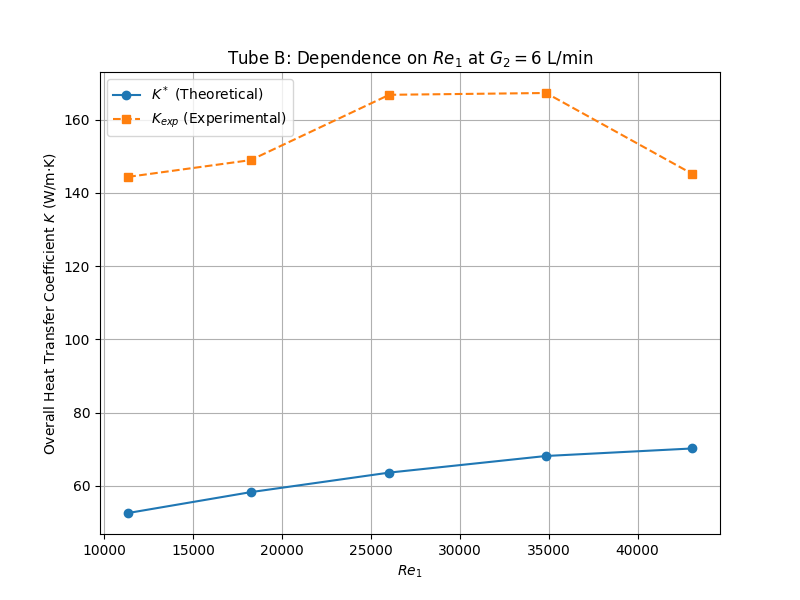
\includegraphics[width=\textwidth]{Figures/plot_6.png}
        \caption{$G_2 = 6$ L/min}
    \end{subfigure}
    \vskip\baselineskip
    \begin{subfigure}[b]{0.48\textwidth}
        \centering
        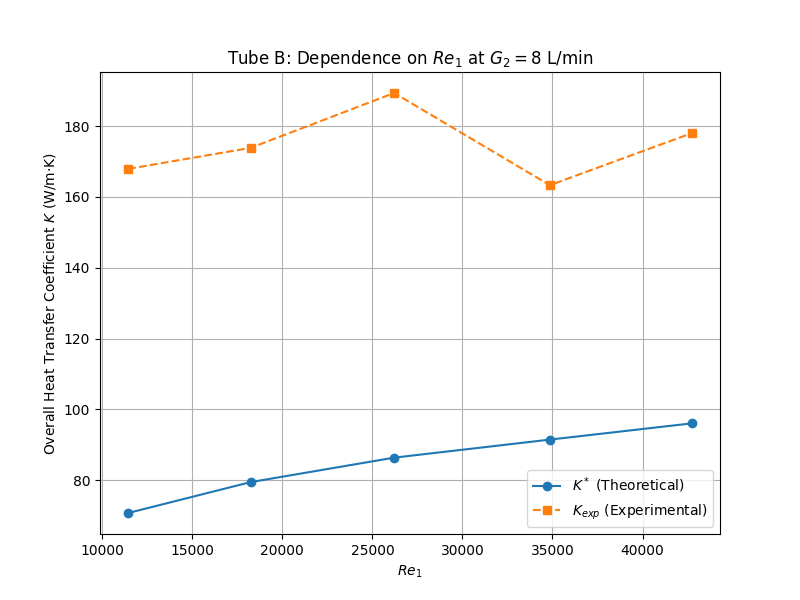
\includegraphics[width=\textwidth]{Figures/plot_7.png}
        \caption{$G_2 = 8$ L/min}
    \end{subfigure}
    \hfill
    \begin{subfigure}[b]{0.48\textwidth}
        \centering
        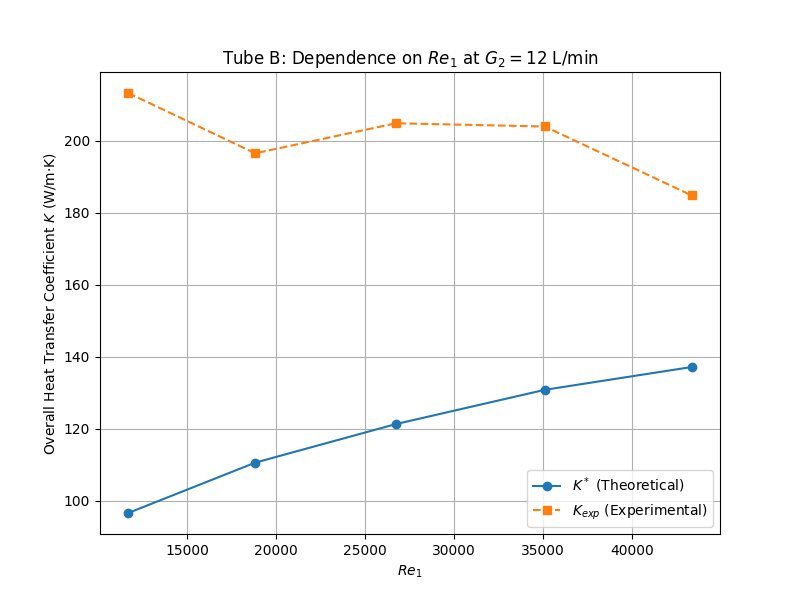
\includegraphics[width=\textwidth]{Figures/plot_8.png}
        \caption{$G_2 = 12$ L/min}
    \end{subfigure}
    \caption{Tube B: Dependence of $K$ on $Re_1$ at varying cold water flow rates $G_2$}
    \label{fig:tube-b-re1}
\end{figure}

\begin{longtable}{|c|c|c|c|}
    \caption{Overall ($K_l^*$) and Experimental ($K_l$) coefficients - Tube C} \label{tab:k-c}                          \\ \hline
    \textbf{No.} & \shortstack{\boldmath$K_l^*$                                              \\ (W/m$\cdot$K)} & \shortstack{\boldmath$K_l$ \\ (W/m$\cdot$K)} & \shortstack{\boldmath$Error$ \\ (\%)} \\ \hline
    \endfirsthead
    \multicolumn{4}{c}{{\bfseries \tablename\ \thetable\ -- continued from previous page}} \\ \hline
    \textbf{No.} & \shortstack{\boldmath$K^*$                                              \\ (W/m$\cdot$K)} & \shortstack{\boldmath$K_{exp}$ \\ (W/m$\cdot$K)} & \shortstack{\boldmath$Error$ \\ (\%)} \\ \hline
    \endhead
    1            & 23.45                      & 96.93  & 75.81                             \\
    2            & 42.21                      & 89.73  & 52.96                             \\
    3            & 55.10                      & 98.19  & 43.89                             \\
    4            & 63.95                      & 109.92 & 41.82                             \\
    5            & 70.83                      & 104.16 & 32.00                             \\ \hline
    6            & 28.03                      & 115.69 & 75.77                             \\
    7            & 50.20                      & 122.02 & 58.86                             \\
    8            & 65.68                      & 119.88 & 45.21                             \\
    9            & 77.98                      & 133.55 & 41.61                             \\
    10           & 87.46                      & 146.78 & 40.42                             \\ \hline
    11           & 30.92                      & 132.30 & 76.63                             \\
    12           & 56.05                      & 137.85 & 59.34                             \\
    13           & 75.11                      & 156.31 & 51.95                             \\
    14           & 88.75                      & 143.32 & 38.08                             \\
    15           & 100.74                     & 158.82 & 36.57                             \\ \hline
    16           & 33.42                      & 137.40 & 75.67                             \\
    17           & 61.04                      & 153.75 & 60.30                             \\
    18           & 81.52                      & 161.30 & 49.46                             \\
    19           & 98.32                      & 169.17 & 41.88                             \\
    20           & 110.97                     & 170.55 & 34.93                             \\ \hline
    21           & 34.77                      & 153.70 & 77.38                             \\
    22           & 64.44                      & 153.57 & 58.04                             \\
    23           & 86.45                      & 174.70 & 50.51                             \\
    24           & 104.72                     & 178.85 & 41.45                             \\
    25           & 119.82                     & 195.48 & 38.70                             \\ \hline
\end{longtable}

\begin{figure}[H]
    \centering
    \begin{subfigure}[b]{0.48\textwidth}
        \centering
        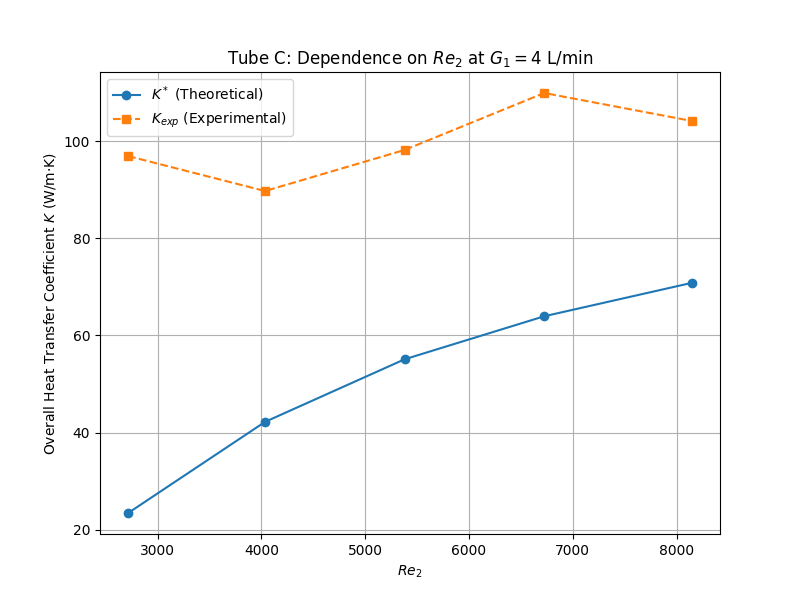
\includegraphics[width=\textwidth]{Figures/plot_9.png}
        \caption{$G_1 = 4$ L/min}
    \end{subfigure}
    \hfill
    \begin{subfigure}[b]{0.48\textwidth}
        \centering
        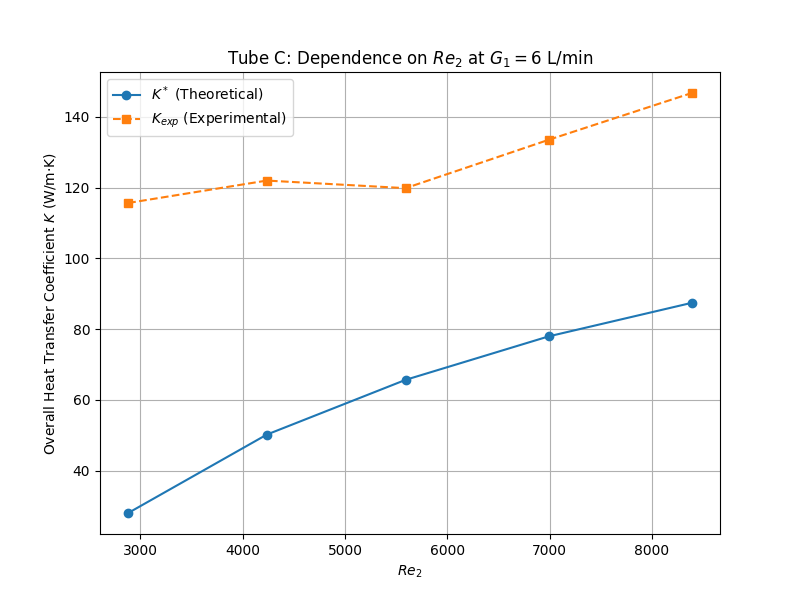
\includegraphics[width=\textwidth]{Figures/plot_10.png}
        \caption{$G_1 = 6$ L/min}
    \end{subfigure}
    \vskip\baselineskip
    \begin{subfigure}[b]{0.48\textwidth}
        \centering
        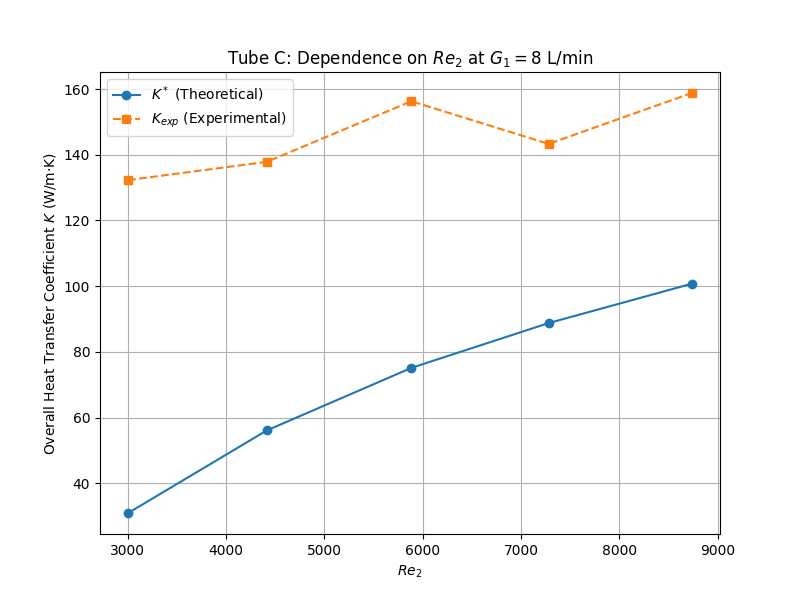
\includegraphics[width=\textwidth]{Figures/plot_11.png}
        \caption{$G_1 = 8$ L/min}
    \end{subfigure}
    \hfill
    \begin{subfigure}[b]{0.48\textwidth}
        \centering
        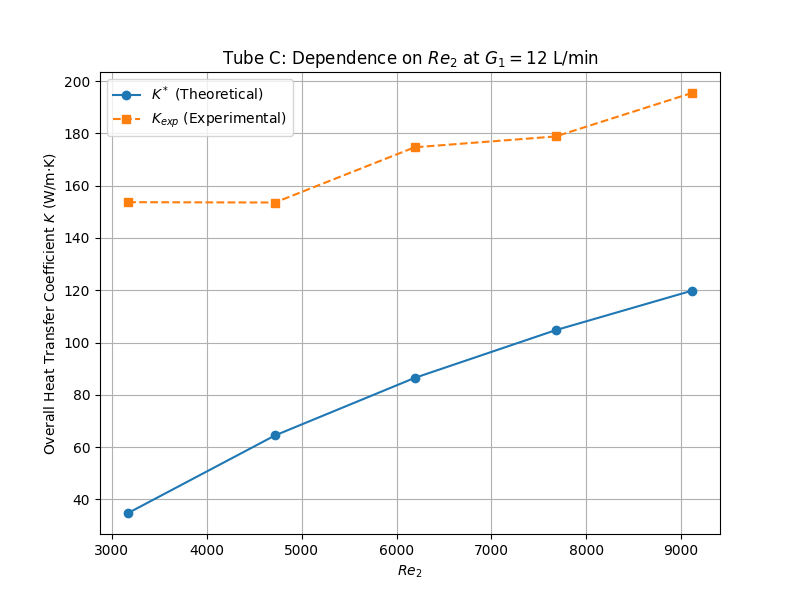
\includegraphics[width=\textwidth]{Figures/plot_12.png}
        \caption{$G_1 = 12$ L/min}
    \end{subfigure}
    \caption{Tube C: Dependence of $K$ on $Re_2$ at varying hot water flow rates $G_1$}
    \label{fig:tube-c-re2}
\end{figure}

\begin{figure}[H]
    \centering
    \begin{subfigure}[b]{0.48\textwidth}
        \centering
        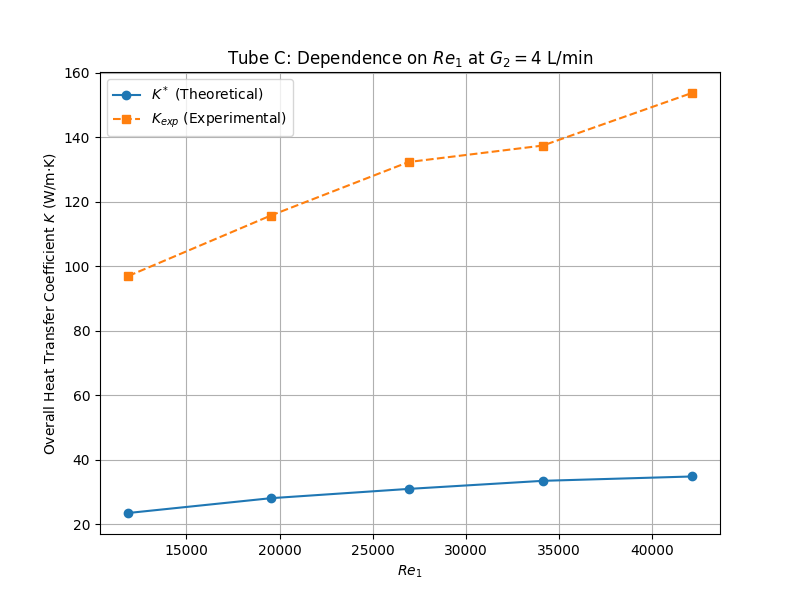
\includegraphics[width=\textwidth]{Figures/plot_13.png}
        \caption{$G_2 = 4$ L/min}
    \end{subfigure}
    \hfill
    \begin{subfigure}[b]{0.48\textwidth}
        \centering
        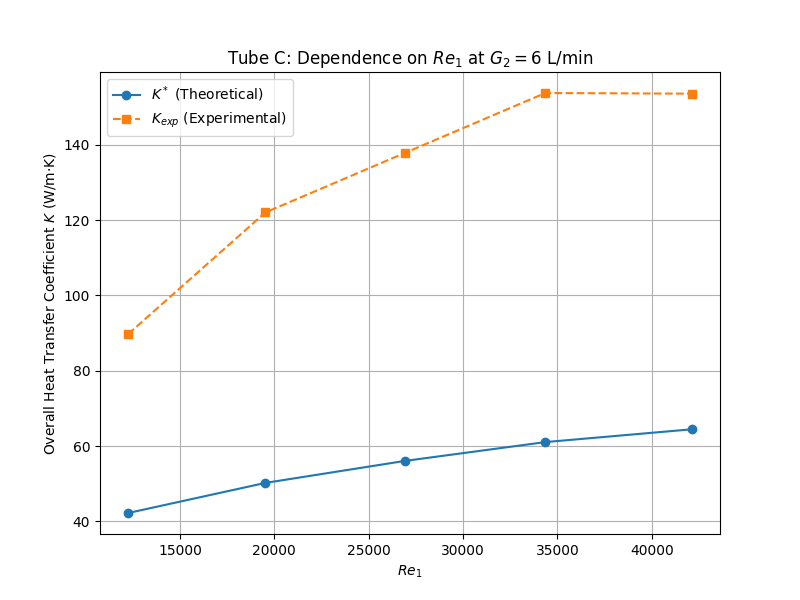
\includegraphics[width=\textwidth]{Figures/plot_14.png}
        \caption{$G_2 = 6$ L/min}
    \end{subfigure}
    \vskip\baselineskip
    \begin{subfigure}[b]{0.48\textwidth}
        \centering
        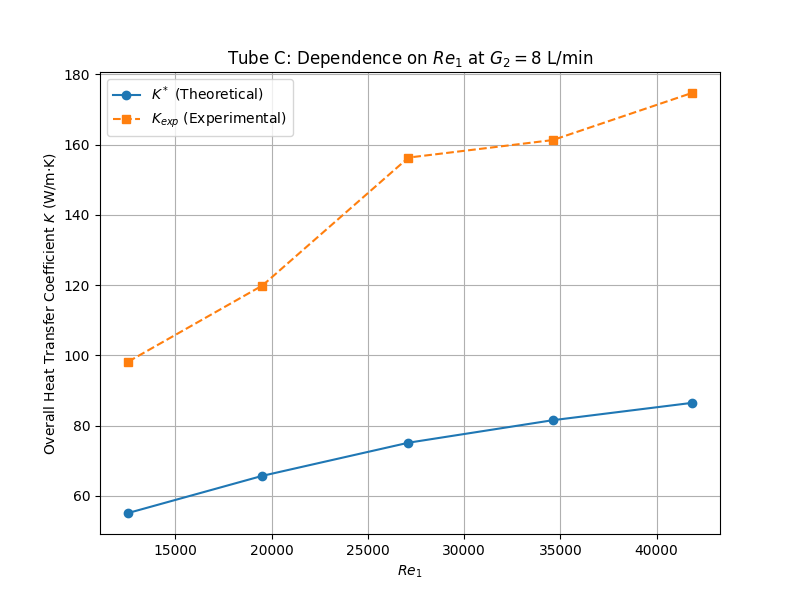
\includegraphics[width=\textwidth]{Figures/plot_15.png}
        \caption{$G_2 = 8$ L/min}
    \end{subfigure}
    \hfill
    \begin{subfigure}[b]{0.48\textwidth}
        \centering
        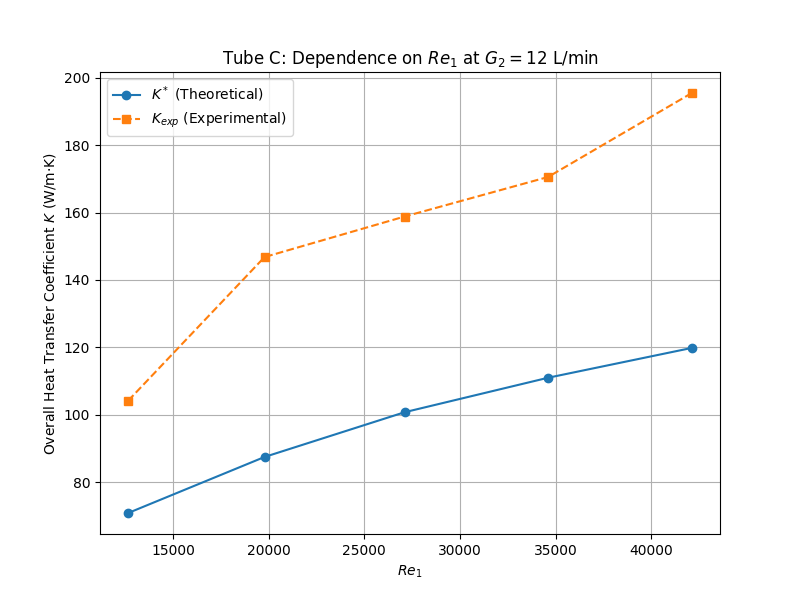
\includegraphics[width=\textwidth]{Figures/plot_16.png}
        \caption{$G_2 = 12$ L/min}
    \end{subfigure}
    \caption{Tube C: Dependence of $K$ on $Re_1$ at varying cold water flow rates $G_2$}
    \label{fig:tube-c-re1}
\end{figure}

\begin{longtable}{|c|c|c|c|c|}
    \caption{Heat transfer coefficients and $K_l^*$ dependence on flow mode - Tube B} \label{tab:dependence-b}                    \\ \hline
    \textbf{No.} & \boldmath$Re_2$ & \shortstack{\boldmath$\alpha_1$                       \\ (W/m$^2\cdot$K)} & \shortstack{\boldmath$\alpha_2$ \\ (W/m$^2\cdot$K)} & \shortstack{\boldmath$K_l^*$ \\ (W/m$\cdot$K)} \\ \hline
    \endfirsthead
    \multicolumn{5}{c}{{\bfseries \tablename\ \thetable\ -- continued from previous page}} \\ \hline
    \textbf{No.} & \boldmath$Re_2$ & \shortstack{\boldmath$\alpha_1$                       \\ (W/m$^2\cdot$K)} & \shortstack{\boldmath$\alpha_2$ \\ (W/m$^2\cdot$K)} & \shortstack{\boldmath$K^*$ \\ (W/m$\cdot$K)} \\ \hline
    \endhead
    1            & 2882.1          & 5297.5                          & 620.1  & 27.4       \\
    2            & 4367.8          & 5057.5                          & 1374.7 & 52.6       \\
    3            & 5764.2          & 4968.1                          & 2091.1 & 70.7       \\
    4            & 7205.2          & 4914.9                          & 2815.6 & 85.1       \\
    5            & 8646.3          & 4870.1                          & 3530.7 & 96.5       \\ \hline
    6            & 3005.2          & 6914.5                          & 686.4  & 30.9       \\
    7            & 4507.8          & 6609.6                          & 1455.5 & 58.3       \\
    8            & 6010.4          & 6466.0                          & 2205.7 & 79.4       \\
    9            & 7433.5          & 6393.3                          & 2935.2 & 96.3       \\
    10           & 8920.2          & 6344.2                          & 3679.1 & 110.5      \\ \hline
    11           & 3171.2          & 8400.2                          & 769.8  & 35.0       \\
    12           & 4680.3          & 8050.5                          & 1549.1 & 63.6       \\
    13           & 6141.7          & 7881.8                          & 2301.9 & 86.3       \\
    14           & 7594.1          & 7765.2                          & 3043.8 & 105.0      \\
    15           & 9112.9          & 7690.3                          & 3800.8 & 121.3      \\ \hline
    16           & 3251.1          & 9601.7                          & 800.8  & 36.7       \\
    17           & 4836.0          & 9390.4                          & 1630.9 & 68.1       \\
    18           & 6291.0          & 9114.7                          & 2371.9 & 91.4       \\
    19           & 7863.8          & 8989.3                          & 3153.3 & 112.4      \\
    20           & 9436.5          & 8933.4                          & 3943.0 & 130.8      \\ \hline
    21           & 3306.7          & 10707.7                         & 821.8  & 37.9       \\
    22           & 4918.0          & 10465.5                         & 1655.3 & 70.2       \\
    23           & 6448.1          & 10276.7                         & 2442.0 & 96.0       \\
    24           & 7993.5          & 10135.0                         & 3221.7 & 118.0      \\
    25           & 9592.2          & 10022.1                         & 4004.8 & 137.1      \\ \hline
\end{longtable}

\begin{longtable}{|c|c|c|c|c|}
    \caption{Heat transfer coefficients and $K_l^*$ dependence on flow mode - Tube C} \label{tab:dependence-c}                         \\ \hline
    \textbf{No.} & \boldmath$Re_2$ & \boldmath$\alpha_1$ & \boldmath$\alpha_2$ & \boldmath$K_l^*$ \\
    \textbf{}    &                 & (W/m$^2\cdot$K)     & (W/m$^2\cdot$K)     & (W/m$\cdot$K)  \\ \hline
    \endfirsthead
    \multicolumn{5}{c}{{\bfseries \tablename\ \thetable\ -- continued from previous page}}      \\ \hline
    \textbf{No.} & \boldmath$Re_2$ & \boldmath$\alpha_1$ & \boldmath$\alpha_2$ & \boldmath$K^*$ \\
                 &                 & (W/m$^2\cdot$K)     & (W/m$^2\cdot$K)     & (W/m$\cdot$K)  \\ \hline
    \endhead
    1            & 2715.5          & 3158.0              & 562.1               & 23.4           \\
    2            & 4034.5          & 2930.1              & 1253.1              & 42.2           \\
    3            & 5379.3          & 2873.5              & 1953.8              & 55.1           \\
    4            & 6724.2          & 2828.3              & 2637.4              & 64.0           \\
    5            & 8146.6          & 2802.5              & 3343.3              & 70.8           \\ \hline
    6            & 2882.1          & 4518.3              & 650.5               & 28.0           \\
    7            & 4236.5          & 4237.5              & 1372.2              & 50.2           \\
    8            & 5592.6          & 4094.4              & 2068.8              & 65.7           \\
    9            & 6990.7          & 4040.2              & 2785.7              & 78.0           \\
    10           & 8388.9          & 4000.1              & 3493.4              & 87.5           \\ \hline
    11           & 3005.2          & 5714.9              & 702.8               & 30.9           \\
    12           & 4413.5          & 5466.1              & 1459.9              & 56.0           \\
    13           & 5884.7          & 5327.3              & 2213.0              & 75.1           \\
    14           & 7279.7          & 5192.4              & 2911.3              & 88.8           \\
    15           & 8735.7          & 5149.0              & 3646.5              & 100.7          \\ \hline
    16           & 3120.2          & 6845.0              & 749.5               & 33.4           \\
    17           & 4606.2          & 6639.0              & 1542.0              & 61.0           \\
    18           & 6075.3          & 6452.8              & 2290.0              & 81.5           \\
    19           & 7594.1          & 6343.8              & 3045.8              & 98.3           \\
    20           & 8920.2          & 6253.1              & 3739.2              & 111.0          \\ \hline
    21           & 3171.2          & 7950.4              & 769.8               & 34.8           \\
    22           & 4718.3          & 7749.1              & 1587.8              & 64.4           \\
    23           & 6190.6          & 7536.2              & 2341.9              & 86.5           \\
    24           & 7677.1          & 7420.2              & 3094.2              & 104.7          \\
    25           & 9112.9          & 7337.8              & 3831.7              & 119.8          \\ \hline
\end{longtable}

